%\documentclass[12pt,fleqn]{amsart} deleted fleqn as I want to have centered equations. Henrik
\documentclass[12pt]{amsart}

\usepackage[T1]{fontenc}
\usepackage[utf8]{inputenc}
\usepackage[margin=1in]{geometry}
\usepackage{amsmath,amssymb,amsfonts}
\usepackage{graphicx,epstopdf}
\usepackage{enumitem}
\usepackage{setspace}
\usepackage{hyperref}

\doublespacing

\title{CS 187 - Dependency Parsing\\Phase 4: Final Paper Draft}
\author{Lauren Urke, Nathaniel Herman, Henrik Sigstad, Ariel Camperi}
\date{}

\begin{document}
    \begin{abstract}
    Utterance structure parsing is a very important area of computational linguistics, as it is a precursor to meaning analyses of utterances. Dependency parsing is one such method which parses an utterance into a structure based on inter-word dependency relationships. This paper presents a method for using Support Vector Machines to deterministically generate this dependency tree.
    \end{abstract}

    \maketitle

\section{Introduction}
The paper we were assigned \cite{yamada2003statistical} proposes that texts in specialized domains such as medical or legal documents are more amenable to word-word dependency analysis than to phrase structure analysis. This is because generating accurate phrase structure parses in these domains requires training models on annotated phrase structure parses of corpora in the relevant domain. This is hard for experts in the relevant domains to do, as it necessitates rather deep linguistic knowledge. Therefore it is much more realistic to have such domain-experts annotate corpora with word-word dependencies, which require only superficial linguistic knowledge.

The method we present in this paper uses Support Vector Machines (described more in detail in further sections) to train a model from annotated Penn treebank data, using a variety of local features for target word pairings. This model is then applied in a bottom-up manner to ``flat'' sentences (i.e. un-annotated with structure) and used to generate a dependency tree. The motivation for this is to see whether a model trained using only word-word dependency data in a given domain is good enough to predict word-word dependencies on an unknown text in that domain.

The paper is organized as follows. First we will describe the method we used in more detail, including an explanation of how we used Support Vector Machines and why they were relevant to the problem, and a explanation of the attached source code. Next we describe the data that was used to train and test this method. Finally, our results are presented and we draw conclusions from them.

\section{Description of the method}
We give a short overview of SVMs based on \cite{hastie2009elements}.
\subsection{Support Vector Machines}


The Support Vector Machine (SVM) is a binary classifier. Assume that the training data consists of $(\mathbf x_i,y_i)$ where $\mathbf x_i \in \mathbb R^p$ are the features and $y_i \in \{-1,1 \}$ for $i \in \{ 1, ..., N \}$. The SVM finds a hyperplane in the feature space which separates the training data according to $y_i$ with the greatest possible margin $M$ allowing for some slack. Specifically it solves the optimization problem
\[ \max_{\beta,\beta_0} M \]
\[ \textrm{ subject to } y_i(x_i^T \beta + \beta_0) \geq M(1- \xi_i) \]
\[ \xi_i \geq 0,\; \sum \xi_i \leq C \textrm{ and } \| \beta \| = 1 \]
where the maximum total amount of slack $C$ is chosen by tuning or by any other method. Here we will follow \cite{yamada2003statistical} and use $C=1$. The classifier is then given by
\[G(x) = \operatorname{sign} [x^T \beta + \beta_0] \]

\begin{figure}
\center
\caption{The Support Vector Machine finds the hyperplane $x^T\beta + \beta_0 = 0$ with $\| \beta \| = 1$ in the feature space which separates the training data with the highest margin $M$ given some slack $\sum \xi_i = C$.}
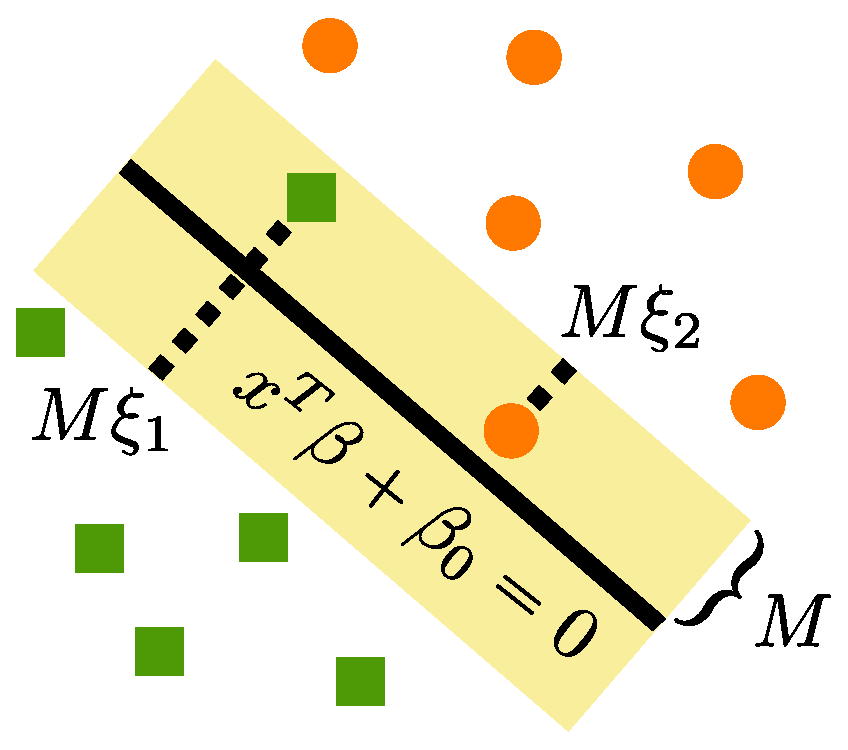
\includegraphics[scale=0.5]{svm.eps}
\end{figure}

In its most basic form the SVM only considers linear hyperplanes in the feature space. However, it is straight forward to introduce non-linearities by transformations of the feature space and applying the basic SVM on this transformed space. Furthermore, it turns out that the classifier depends only on inner products between pairs of observations in the transformed space. The inner product in the transformed space is called the \emph{kernel function}. Instead of specifying the transformation itself it is therefore customary to only state the kernel function. A common kernel is the polynomial kernel
\[ K(x,x')=(1+ <x,x'> ) ^d \]

This is the kernel employed by \cite{yamada2003statistical}.

The SVM can be extended to multi-class classification problems in several ways. One possibility is to train an SVM for each pairs of classes, and then let final classifier be the one that dominates the most. We will refer to this as \emph{one-vs-one} SVM. Another possibility is to train binary SVMs of each class against the rest of the classes, and choose the classifier which gives the highest margin. We refer to this as the \emph{one-vs-the rest} SVM. A third, alternative which is claimed to have a better theoretical foundation, but is more computationally expensive is the Crammer-Singer multiclass SVM \cite{crammer2002algorithmic}.

SVMs are great in our context as they are able to use a very high dimensional feature space (e.g. all neighboring words and POS tags) even allowing for interdependencies relatively cheaply.


\subsection{Description of dependency parsing}

Dependency grammar is a way of analysis syntax in terms of dependency relations between words, as opposed to phrase structure grammar which analyses sentences in terms of constituencies (e.g. noun phrases and verb phrases). Typically the root node is the main verb in the sentence and dependencies are built around this node based on different rules. As seen in Figure \ref{dep} dependency grammars are much simpler than constituency grammars.
\begin{figure}
\center
\label{dep}
\caption{Constituency versus dependency grammar}
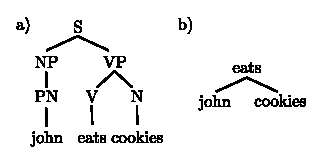
\includegraphics[scale=1.5]{dep.eps}
\end{figure}

\subsection{Description of Code}
Our actual implementation uses the same basic parsing algorithm as that in 
\cite{yamada2003statistical} (i.e. Figure 6 of the paper). Essentially, we look at
2 elements of our array (which is initially the list of words in a sentence)
at a time, using the contextual features (like POS tags) to estimate
the relation (Left, Right, or Shift) to use between the 2 elements. 

Of course, the hard part of the implementation is not in writing the basic 
parsing algorithm, but
rather in writing the get\_contextual\_features(), estimate\_action(),
and construction() functions
to work correctly for both the training phase and prediction phase (as well
as generating the SVM(s) themselves and saving them to disk).

Our array (the ``T'' variable in \cite{yamada2003statistical}) 
starts as an array of words, which are really
dictionaries describing a given word's features like its POS. As we construct
child-parent relations, the array elements become trees themselves representing
these child-parent relations. To make an element the child of a tree, we append 
the element to the tree's list of children.

get\_contextual\_features() works the same whether we're training or predicting,
and simply creates a dictionary which maps various information tuples 
(including information about a tree's children, and contextual information) to
1's. For instance we might have a dictionary (in Python) that looks something 
like:
\begin{verbatim}
{(0, 'pos', 'NP'): 1, (0, 'lex', 'resort'): 1,
  (0, 'ch-R-pos': 'JJ'): 1, (0, 'ch-R-lex': 'last'): 1}
\end{verbatim}
This specific format is to make it easily convertible to a matrix of 1's and 
0's for our SVM.

For the training phase, estimate\_action() works as follows: we look to see if
the two nodes in consideration have an actual parent-child relation to each 
other (in the training dataset). If so, we choose Left or Right as our action 
to construct this parent-child relation. However, once a node is made the 
child of another node, we can no longer add any children to it. Thus, we only
pick Left or Right if the node which will become child has already had all of
its own children added to it. In all other cases we pick Shift as our action.

The training model also keeps track of a list of its decisions. We store both
what action it picks, as well as what the contextual features were for that
particular action choice. Thus, once the training model has been run on the
data, we can construct an SVM which associates sets of contextual features 
with actions, and store it to disk (so we don't have to retrain each run
through).

Then we can run our predictor model on test data, where estimate\_action()
now predicts what action to take using our SVM with the contextual
features at the current location in the sentence.

In our full implementation, we actually use multiple SVMs, one per POS tag.
Thus to predict the action for the ith element in our array, we use the SVM
associated with whatever part of speech the ith word in the array is. This
makes it more tractable to run our data with very large datasets (the Penn
treebank dataset is fairly large) so we don't end up with one gigantic SVM.

\section{Description of Data}
To implement Dependency Parsing, we used the Penn Treebank Project Data. The treebank data contains sentences that have been parsed into a linguistic trees that also contain part-of-speech tagging.

Parsed in this way, "Pieere Vinken, 61 years old, will join the board as a non executive director Nov. 29.", will look like this: 
\begin{verbatim}
( (S
         (NP-SBJ 
               (NP (NNP Pierre) (NNP Vinken) )
               (, ,) 
               (ADJP
                       (NP (CD 61) (NNS years) )
                       (JJ old) )
                (, ,) )
         (VP (MD will) 
               (VP (VB join) 
                       (NP (DT the) (NN board) )
                       (PP-CLR (IN as) 
                             (NP (DT a) (JJ nonexecutive) (NN director) ))
                       (NP-TMP (NNP Nov.) (CD 29) )))
         (. .) ))\end{verbatim}

This information is helpful, but could be improved. To conduct analysis on the dependencies, we wanted to be able to easily infer the relationship between two words. Therefore, we used a program from the Lund University Computer Science Department that converted the Penn Treebank parses into dependency parses. For each word in a sentence, a dependency parse indicates the parent word and the part of speech. For example, the same sentence now comes out as in Table \ref{dependency_parse}.

\begin{table}
\label{dependency_parse}
\caption{Dependency parse}
        \begin{tabular}{ccccc}
\hline \hline
            ID & Token & Part of Speech & Parent ID & Class \\ 
            \hline
            1 &Pierre & NNP & 2 & NAME \\
            2 & Vinken & NNP & 8 & SBJ\\
            3 & , & , & 2 & P\\
            4 & 61 & CD & 5 & NMOD\\
            5 & years & NNS & 6 & AMOD\\
            6 & old & JJ & 2 & APPO\\
            7 & , & , & 2 & P\\
            8 & will & MD & 0 & ROOT\\
            9 & join & VB & 8 & VC\\
            10 & the & DT & 11 & NMOD\\
            11 & board & NN & 9 & OBJ\\
            12 & as & IN & 9 & ADV\\
            13 & a & DT & 15 & NMOD\\
            14 & nonexecutive & JJ & 15 & NMOD\\
            15 & director & NN & 12 & PMOD\\
            16 & Nov. & NNP & 9 & TMP\\
            17 & 29 & CD & 16 & NMOD\\
            18 & . & . & 8 & P\\
            \hline
        \end{tabular}
\end{table}

This data now directly tells us the parental relationships between two words in a sentence. The Penn Treebank contains 24 sections. We used sections 02-22 for training and section 23 for testing. Section 23 contains 2,416 sentences, which includes 56,684 words (49,892 without punctuation).

\section{Results}
We used three measurements to evaluate the effectiveness of this method.
\begin{eqnarray*}
    \text{Dependency Accuracy} &=& \dfrac{\text{number of correct parents}}{\text{total number of parents}}\\
    \text{Root Accuracy} &=& \dfrac{\text{number of correct root nodes}}{\text{total number of sentences}}\\
    \text{Complete Rate} &=& \dfrac{\text{number of complete parsed sentences}}{\text{total number of sentences}}
\end{eqnarray*}
Using a default context of (2,2), we evaluated two different linear multiclass SVCs. The results for the One vs One and a One vs Many respectively is presented in Table \ref{key_results}.
\begin{table}
\label{key_results}
\caption{Results for linear multiclass SVCs using a context length of (2,2)}
        \begin{tabular}{c|ccc}
            \hline \hline Dependency Accuracy & Root Accuracy & Complete Rate \\ \hline
            One vs one SVC & 0.89135 & 0.93675 & 0.32711 \\
            One vs many SVC & 0.88680 & 0.93894 & 0.32285 \\ \hline
        \end{tabular}
\end{table}
The Sci-kit Learn offered several other SVM options, but after testing each of them with a set context length, we determined
that none of them improved our results. We then empirically determined the optimal context length for the One vs One classifier. The Context determines how many words to the left and right of the target nodes are considered.
\begin{table}
\caption{Varying the context length}
\begin{tabular}{l|cccc|cccc}
  \hline \hline
&\multicolumn{8}{c}{context length} \\ \hline
             & (2,2) & (2,3) & (2,4) & (2,5) & (3,2) & (3,3) & (3,4) & (3,5) \\ \hline 
            Dep. Acc. & 0.891 & 0.890 & 0.890 & 0.889 & 0.887 & 0.887 & 0.887 & 0.887 \\
            Root Acc. & 0.937 & 0.928 & 0.934 & 0.930 & 0.932 & 0.929 & 0.928 & 0.927 \\
            Comp. Rate & 0.327 & 0.330 & 0.325 & 0.326 & 0.312 & 0.318 & 0.316 & 0.317 \\ \hline
\end{tabular}
\end{table}
We determined that the One vs One Linear SVC gave the best results when used with a context of 2 on either side of the target nodes. 

\section{Conclusion}
Yamada and Matsumoto's implementation of dependency parsing used a One vs One classifier to parse the sentences. They tested different kernel degrees, and ended up with a quadratic kernel. They determined that a context of 2 on the left and 4 on the right was best (for dependency accuracy). This is slightly different from our results, however the differences here are quite small, with ours getting 89.0% accuracy for (2,4) versus 89.1% accuracy for (2,2) and their results getting 90.3% for (2,4) and 90.0% for (2,2). Their quadratic implementation gave only slightly better results than our linear implementation, while their linear implementation did worse than ours:       \\
\begin{table}
\caption{Comparison of results}
 \begin{tabular}{cccc}
            \hline \hline & Dependency Accuracy & Root Accuracy & Complete Rate \\ \hline
            Y and M Quadratic & 0.900 & 0.896 & 0.379 \\ 
            Y and M Linear & 0.854 & 0.811 & 0.261 \\ 
            Our Linear Results & 0.89135 & 0.93675 & 0.32711 \\
            \hline

        \end{tabular}
\end{table}
Our implementation successfully modeled Yamada and Matsumoto's dependency parsing algorithm with fairly similar results on the linear kernel level. In theory, a One vs Many classifier should work better than a three-part One vs One classifier. Possible next steps to improve results include investigating other One vs Many classifiers and attempting to pinpoint why this classifier did not improve parsing accuracy. Another possible next step includes testing out various other kernel functions.
        
\bibliographystyle{plain}
\bibliography{ref}
        

%\begin{thebibliography}{1}
%\bibitem{original-paper}$\textsc{Yamada, H., and Matsumoto, Y.}$ Statistical Dependency Analysis With Support Vector %Machines. In \emph{Proceedings of IWPT}, 2003.
%\end{thebibliography}

\end{document}

%%% Local Variables:
%%% mode: latex
%%% TeX-master: t
%%% End:
